% Las 5 G's del Geometric Deep Learning
% Compilar con: pdflatex five_gs_framework.tex
\documentclass[tikz,border=10pt]{standalone}
\usepackage{tikz}
\usetikzlibrary{shapes.geometric, arrows.meta, positioning, shadows, calc}

\definecolor{gdlblue}{RGB}{41, 98, 168}
\definecolor{gdlred}{RGB}{191, 49, 49}
\definecolor{gdlgreen}{RGB}{30, 130, 76}
\definecolor{gdlorange}{RGB}{217, 130, 30}
\definecolor{gdlpurple}{RGB}{118, 56, 138}
\definecolor{gdlgray}{RGB}{140, 140, 140}
\definecolor{gdlyellow}{RGB}{190, 140, 10}

\begin{document}
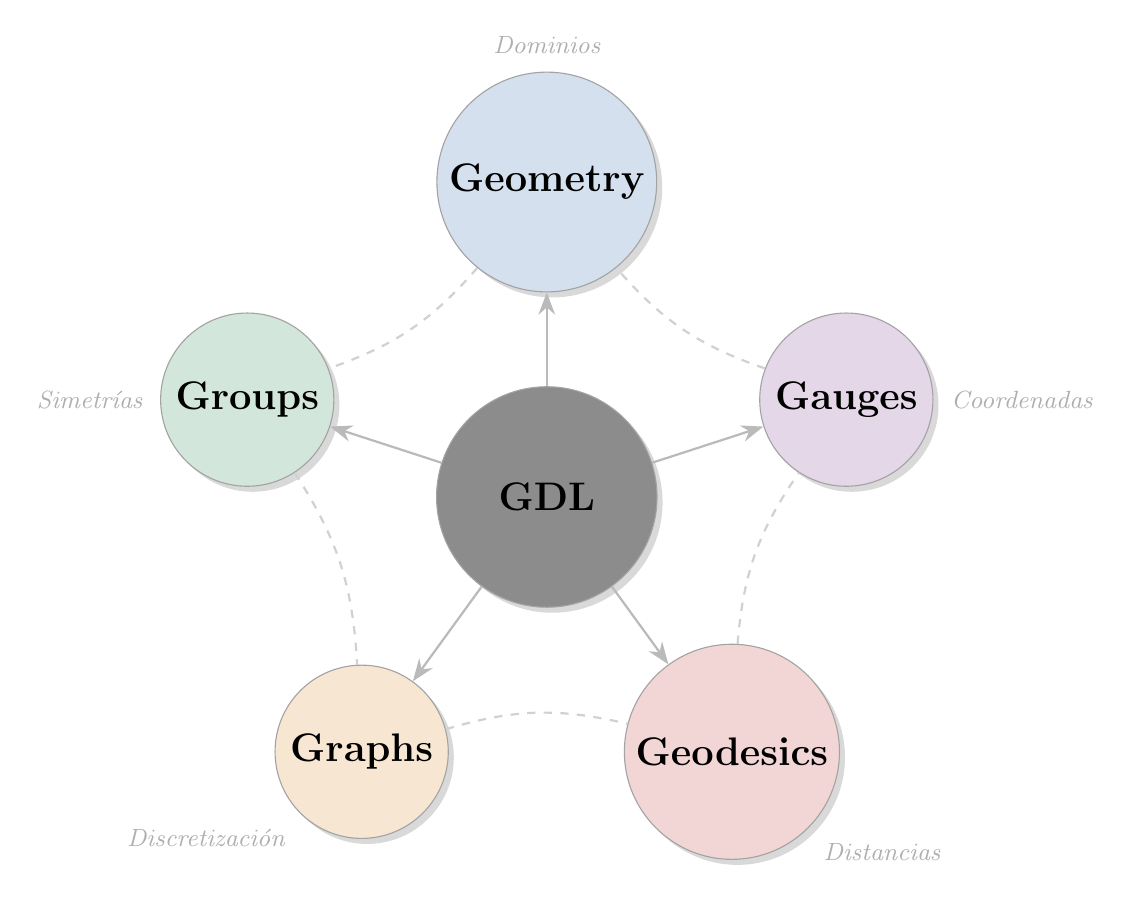
\begin{tikzpicture}[
    node distance=1.8cm,
    gnode/.style={
        circle,
        draw=gdlgray!80,
        fill=#1,
        minimum size=2.2cm,
        font=\bfseries\Large,
        drop shadow={shadow xshift=2pt, shadow yshift=-2pt, opacity=0.3}
    },
    arrow/.style={-{Stealth[length=8pt]}, thick, draw=gdlgray!60},
    label/.style={font=\small\itshape, text=gdlgray!70}
]

% Central node
\node[gnode=gdlgray, minimum size=2.8cm] (gdl) at (0,0) {GDL};

% 5 G's around the center
\node[gnode=gdlblue!20] (geometry) at (90:4cm) {Geometry};
\node[gnode=gdlgreen!20] (groups) at (162:4cm) {Groups};
\node[gnode=gdlorange!20] (graphs) at (234:4cm) {Graphs};
\node[gnode=gdlred!20] (geodesics) at (306:4cm) {Geodesics};
\node[gnode=gdlpurple!20] (gauges) at (18:4cm) {Gauges};

% Arrows from center to G's
\draw[arrow] (gdl) -- (geometry);
\draw[arrow] (gdl) -- (groups);
\draw[arrow] (gdl) -- (graphs);
\draw[arrow] (gdl) -- (geodesics);
\draw[arrow] (gdl) -- (gauges);

% Labels for each G
\node[label, above=0.1cm of geometry] {Dominios};
\node[label, left=0.1cm of groups] {Simetrías};
\node[label, below left=0.1cm of graphs] {Discretización};
\node[label, below right=0.1cm of geodesics] {Distancias};
\node[label, right=0.1cm of gauges] {Coordenadas};

% Connecting arcs between G's (showing relationships)
\draw[thick, dashed, draw=gdlgray!40] (geometry) to[bend left=15] (groups);
\draw[thick, dashed, draw=gdlgray!40] (groups) to[bend left=15] (graphs);
\draw[thick, dashed, draw=gdlgray!40] (graphs) to[bend left=15] (geodesics);
\draw[thick, dashed, draw=gdlgray!40] (geodesics) to[bend left=15] (gauges);
\draw[thick, dashed, draw=gdlgray!40] (gauges) to[bend left=15] (geometry);

\end{tikzpicture}
\end{document}
